%proo\documentclass[acmtog,nonacm]{acmart}
\documentclass{tstextbook}
\usepackage{tikz}
\usetikzlibrary{decorations.pathreplacing,positioning,chains, shapes.geometric}
\usepackage{tipa}
\usepackage{color}
\usepackage{listings}
\makeatletter
\def\lmtt@use@light@as@normal{}
\usepackage{etoolbox}
%\usepackage{amsmath}
%\theoremstyle{plain}% default
%\newtheorem{thm}{Theorem}[section]
%\newtheorem{prop}[thm]{Proposition}
%\theoremstyle{definition}
%\newtheorem{defn}{Definition}[section]

\usepackage{booktabs}

\input{vc.tex}


\usepackage[lastexercise,answerdelayed]{exercise}
\setlength{\Exesep}{.5ex}
\setlength{\Exetopsep}{1em}
\renewcommand{\ExerciseListName}{Exercise}
\renewcommand{\AnswerListName}{}
\renewcommand{\ExerciseHeaderTitle}{(\emph{\ExerciseTitle.})\ }
\renewcommand{\ExerciseListHeader}{\ExerciseHeaderDifficulty%
\textbf{\ExerciseListName\ExerciseHeaderNB.}\ \ExerciseHeaderTitle%
\ExerciseHeaderOrigin\ignorespaces}
\renewcommand{\AnswerListHeader}{\textbf{\ExerciseHeaderNB.\ }}

\title{Additional Note for Algorithms and Data Structures}
\author{Thore Husfeldt}
\date{\small Revision {\tt \GITAbrHash}$\ldots$, \GITAuthorDate, \GITAuthorName}
\begin{document}
\maketitle

\chapter{Amortisation}
\label{sec-1.1}
  \begin{summary}
    This note covers the technique of amortized analysis, as a
  supplement to [SW], the textbook \emph{Algorithms, 4th ed.} by
  Sedgewick and Wayne.

  It contains a complete answer to [SW, exercise 1.4.32] thus completing the
  proof of proposition~E in [SW, section 1.4].
  
  It also contains amortised analyses of some union--find data structures.
  \end{summary}

  \section{Aggregate method}
Consider the resizing array implementation of {\tt Stack} (Algorithm 1.1) and the collowing claim:

\begin{theorem}[Proposition E in SW 1.4, only for push]
  \label{prop: E original}
  In the resizing array
  implementation of {\tt Stack} (Algorithm 1.1), the average number of
  array accesses per operation for any sequence of {\tt push()} operations starting
  from an empty data structure is constant in the worst case.
\end{theorem}

This is a true statement, and proved in [SW].
We include a full proof below, in section~\ref{sec: nopop}, just for completeness.

\begin{ExerciseList}
  \Exercise
  Is Prop.~\ref{prop: E original} still true when I remove ``starting from an empty data
structure''?
\Answer
No.
To see this, begin with a stack that is the result of $2^k-1$
applications of {\tt push(null)}. 
Now {\tt N} equals $2^k-1$ and {\tt  a.length} equals $2^k$. 
From this starting position, a single {\tt push()} will result in
a call to {\tt resize()}, leading to a  number of array accesses that is
linear in {\tt N}.
  \Exercise
  Is Prop.~\ref{prop: E original} still true when I remove ``average''?
\Answer
No.
\end{ExerciseList}

 

\section{Terminology: Amortisation versus average}

From now on, we will try to avoid the term ``on the average.'' 
Not because it is wrong, but because it is too broad.
For more precision, we introduce the concept of ``amortised cost'',
borrowing terminology from the world of finance.\footnote{
{\bf amortize} 
/\textipa{"\ae m@r""taIz}, \textipa{@"mOrtaIz}/
verb [trans.]
reduce or extinguish an amount by money regularly put aside:
\emph{loan fees can be amortized over the life of the mortgage.}, gradually write off the initial cost of an asset: \emph{they want to amortize the tooling costs quickly}.
}
\footnote{Many people view this material as  difficult, subtle, and somewhat
boring. It may be well
characterised by a word whose latin root is \emph{ad mortis}, ``to death.''}

The idea is to ``write off'' the costs for {\tt reduce()} in the long
run by showing that, even though a particular call may be costly,
these expensive calls happen with such low frequency that by instead
charging a slight cost to every operation, the expensive operation
will be paid.

As with many good analogies, there is a pitfall: 
In banking it is perfectly acceptable to expend a large amount of
money immediately, and amortise it later, for example, buying a house
off a large loan, or amortising the expense of a good-quality tool
after many uses.
In contrast, this is not acceptable in the analysis of algorithms:
We will insist that every expensive operation is already paid (in
small rates) beforehand.\footnote{Another place where the banking
  analogy breaks down is that banks charge interest. Algorithms don't.}
Maybe ``piggy bank'' analysis would have been a better term, but the
word is what it is.

So, to be quite precise, here is the definition:

  \begin{definition}[Amortized cost]
    Let $T(N)$ be the worst-case\footnote{
      Imagine that the sequence of operations, including the parameters to these operations, are chosen by your worst enemy.}
    total running time for any sequence of $N$ operations.
    The \emph{amortized} time for each operation is $T(N)/N$.
\end{definition}

So why don't we just call it ``average'' time?

Because ``average'' also means many other things. 
For instance, we could average over operations (say, call {\tt push()} and {\tt pop()} with equal probability, and with random arguments to {\tt push()})---this is called ``average case complexity'', and a difficult and active reseach area.
Also, for algorithms that use randomness, we could average over tho random choices of the algorithm---this is called ``expected running time'', another active research area.
Both of these concepts of average make sense for a single opeation, and both would require us to be quite precise about the random processes involved.

In contrast, ``amortized time'' is a particular, precise, worst-case average over a sequence of operations.

\begin{ExerciseList}
  \Exercise
  Bob is a reluctant runner. 
  He has been running 4~km every day of the week, except in the week-ends.
  (i) What is the worst case number of kilometers he runs per day?
  (ii) He started this new workout schedule on a Saturday.
  What is the amortised number of kilometers he runs per day?
  \Answer (i) 4 km per day.
  (ii) When we measure on the $w$th Friday (the worst possible day) we get $(0+0+4+4+4+4+4)w$ kilometers in total, for $7w$ days, which means $\frac{20}{7}<2.9$ kilometers amortised.
  \Exercise
  Ran is also a reluctant runner.
  He rolls a die every morning and runs as many kilometers.
  (i) What is the expected number of kilometers Ran runs per day, assuming he has a perfect die?
  (ii) What is the worst-case number of kilometers Ran runs per day?
  (iii) For any sequence of days starting on a Saturday, what is the worst-case amortised number of kilometers Ran runs per day? (Note that this answer must hold \emph{even if his dice are cursed}.)
  \Answer
  (i) $\frac{7}{2}$. (ii) $6$. (iii) $\frac{5\cdot 6}{7} = \frac{30}{7} \sim 4.28$.
  \Exercise
  My phone company charges 10 DKK for 1 minute of voice call.
  This is exorbitant, but I never use my phone for making a phone call anyway.
  According to the contract, I have to pay at least 100 DKK per month for voice calls whether I use them or not, but the contract automatically `rolls over' the unused minutes to the next month.
  I have call my mum for Christmas for a 2-hour call.
  Describe the expense in terms of `money I spend on voice calls each month' in the worst case and in the amortised sense.
  \Answer
  In the worst month (December), I spend 1200 DKK (which are indeed removed from my account of unused talk minutes at the phone company).
  In the amortized sense, I spend 100 DKK per month (which are indeed removed from my bank account).
  If you want to be precise, the contract must have started in January.
  \Exercise 
  A multiride ticket in the Danish amusement part Tivoli costs 200 DKK and is valid for 10 rides. 
  What is the worst case cost for a single ride? 
  What is the amortised cost for a ride?  
  (\emph{Careful!})
\end{ExerciseList}


\section{Aggregate method}

\section{Stack without Popping}
\label{sec: nopop}

\begin{theorem}[Proposition E in {[SW 1.4]}, reformulated]
  \label{prop: E half}
  In the resizing array
  implementation of {\tt Stack} [SW, Algorithm~1.1], the push operation 
  requires amortised constant time.
\end{theorem}
\begin{proof}
  Starting from an empty data structure, consider any sequence of push operations of length $k$.
  Our cost model is the number of array accesses.
  The second line in the body of \texttt{push} always takes exactly one array acccess, for a total of $k$ accesses.

  The difficult part are the array accesses resulting from the calls to \texttt{resize}.
  A call to \texttt{resize}$(m)$ when the data structure contains $N$ elements requires $m+2N$ array accesses.
  When \texttt{resize} is called from \texttt{push}, we have $m = 2N$, so $m+2N=4N$.
  Such a call happens when $N$ is a power of $2$, i.e., for $N=1$, $2$, $4$, $8$, $\cdots$, $k'$,
  where $k'$ is the largest power of $2$ such that $k'\leq k$.
  In summary, the array accesses resulting from calls to resize result in at most
  \[ 4(1 + 2 + 4 + 8 + \cdots + k') = 4(2k'-1)\leq 8k\,\] 
  array accesses.
  We conclude that the total number of array accesses for any sequence of $k$ calls to \texttt{push} is $9k$.
\end{proof}

\section{Mechanical Counter}

Whenever a mechanical counter is incremented, the rightmost wheel (the
``ones'') is turned. Every 10th increment, when the rightmost wheel
transitions from 9 to 0, its left neighbour is turned as well. This
effect continues to the left, so after $10^k-1$ increments, when the
counter shows $k$ many 9s, the next increment will lead $k+1$ wheels to
turn.

\begin{figure}[htb]
  \centerline{\includegraphics[width=3in]{Zaehlwerk_Schema_1.jpg}}
  \centerline{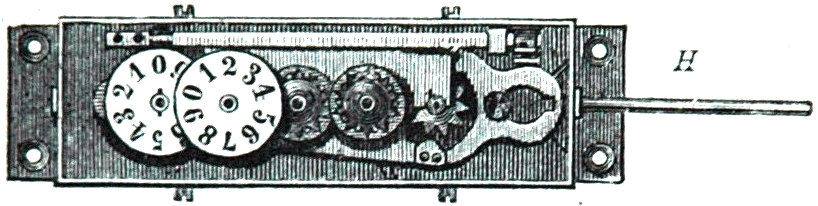
\includegraphics[width=3in]{Zaehlwerk_Schema_2_clean.png}}
\caption{A 5-digit mechanical counter.}
\end{figure}

In our terminology, the worst case number of operations for $N$
increments is logarithmic. But in the amortised sense, the behaviour
is much better:

\begin{theorem}
    Starting from 0, a mechanical counter needs a
  constant amortised number of operations per increment.
\end{theorem}

\begin{proof}
Consider a sequence of $N\geq 0$ increments. 
  Some of them will turn exatly 1 wheel (namely the rightmost), others will turn more wheels.
  The trick is and to look at each wheel separately.
  Enumerate the  wheels $0,\ldots, k-1$ from right to left, so wheel~$0$ shows the least significant digits.  
  Note that the number of wheels needed is exactly the number of digits of $N$ (in the decimal representation), which is  $k=\lfloor \log_{10} N\rfloor + 1$.

Wheel $0$ was rotated $N$ times. 
  Wheel $1$ was rotated $\lfloor N/10\rfloor$ times.
  In general, wheel $r$ was turned \[ \left \lfloor \frac{N}{10^r} \right\rfloor\quad\text{times}\qquad (0\leq r < k)\,.\]
  Adding these contributions for the total number of operations, gives 
\begin{multline*}
 \left \lfloor
\frac{N}{10^0} \right\rfloor +
 \left \lfloor
\frac{N}{10^1} \right\rfloor +
\cdots +
 \left \lfloor
\frac{N}{10^{k-1}} \right\rfloor
\leq \\
\frac{N}{10^0} +
\frac{N}{10^1} +
\cdots +
\frac{N}{10^{k-1}} 
  =
N\left(\frac{1}{10^0}+\frac{1}{10^1}+\cdots+\frac{1}{10^{k-1}} \right) =\\
  N\left(1 + \frac{1}{10} + \frac{1}{100} + \cdots +\frac{1}{10^{k-1}} \right)
< 2N.
\end{multline*}
This finishes the proof.
\end{proof}

\begin{ExerciseList}
  \Exercise{}
  Repeat the above argument, but for a \emph{binary} counter.
  (Every wheel contains only two digits, $0$ and $1$.)
  \Answer
  Now $k=\lceil \log_2 N\rceil + 1$.
  The total number of rotations becomes $\lceil N/2^0\rceil+ \cdots+ \lceil N/2^{k-1}\rceil  \leq N/(1 + \frac12 + \frac14 + \frac18 +\cdots )= 2N$. 
\end{ExerciseList}

\section{Accounting method}

What we will do now is to show that Prop.~\ref{prop: E half} is still true when I remove ``{\tt push()}'':

\begin{theorem}[Proposition E in SW 1.4 in full, reformulated]
  \label{prop: E}
  In the resizing array
  implementation of {\tt Stack} (SW Algorithm 1.1), the amortized number of
  array accesses per operation is constant in the worst case.
\end{theorem}

So now the claim is stronger; it talks about any sequence of operations (including pops), instead of only pushes.
Intuitively, the claim  sounds reasonable, since {\tt pop()} only makes the
stack smaller, whereas the really expensive operation happens only when
the stack grows and causes and expensive {\tt resize()}.
However, even though this argument sounds reasonable, it is \emph{wrong}.
The next section shows why.
\section{Stingy resizing array}
\label{sec-1.2}

We will change algorithm~1.1 to halve the size of {\tt a} as soon as
it can.  
More specifically, let algorithm~1.1' be the same as algorithm 1.1,
with the following change in the implementation of {\tt pop()}, where
a {\tt 4} was replaced by a {\tt 2}.
To be quite precise, we change the line
\begin{quote}
  {\tt if (N > 0 \&\& N == a.length/4) resize(a.length/2);}
\end{quote}
to 
\begin{quote}
  {\tt if (N > 0 \&\& N == a.length/2) resize(a.length/2);}
\end{quote}
   
Note that the implementation remains \emph{correct} (in the sense that it correctly implements a stack), and it will even save space. 
However, we can no longer guarantee the performance of Prop.~\ref{prop: E}.

\begin{ExerciseList}\small
  \Exercise{}
  Exhibit a sequence of operations for which algorithm~1.1' requires a quadratic number of array accesses.
\end{ExerciseList}

In other words, the sequence of operations from the preceding exercise requiers a linear number of array accesses \emph{per operation} on the average, much worse than the constant number
promised by Prop.~\ref{prop: E}.
We must resign ourselves to the fact that Prop.~\ref{prop: E} does not hold for algorithm~1.1'.
Since it does hold for algorithm~1.1, the argument needs to become quantitative somewhere---it must acknowledge the difference between 4 and 2.
Our intuitive argument was purely qualitative, so it can't work.

\section{Amortized Analysis of Resizing Array}

We rephrase the claim with our new terminology:

\begin{theorem}[Prop 1.1, rephrased]
  In the resizing array implementation of {\tt Stack} (Algorithm 1.1),
  the amortised number of array accesses per operation for any
  sequence of operations starting from an empty data structure is
  constant in the worst case.
\end{theorem}
\begin{proof}
We will pretend that every array access costs one coin.  
We associate a (ficticious) piggy bank with our data structure and
make every call of {\tt push()} and {\tt pop()} deposit a certain
number of coins in the bank.  
(Determining how many coins is the technically difficult part of the
argument.) 
The aim is to have the pig bank-roll every call of {\tt resize()}.

Let my pull the right constants out of my hat: {\tt push()} shall
deposit 8 coins, {\tt pop()} shall deposit 4 coin.%
\footnote{If you want to be precise {\tt push()} costs 9 coins. %
  It uses 1 coin to pay for the array access in line 2, and puts the
  others in the pig. %
  Similarly, {\tt pop()} costs 6 coins. %
  It uses 2 coins to pay for the array acccesses in its first two
  lines and puts the remainder in the pig.}

The difficulty are the two internal calls to {\tt resize()}.  
A call to {\tt resize(max)} requires $\mathtt{max}+ 2N$ array
accesses.\footnote{See the last Q\&A in section~1.4 for our convention
  about the cost of {\tt new}.}  
We can simplify this expression by observing that $\mathtt{max}=2N$
whenever {\tt resize()} is called.
To see this, look at the condition to $\mathtt{if}$ in both calls to
\texttt{resize()}: from inside \texttt{push()}, we have $\mathtt{max}=
\mathtt{2*a.length} = 2N$, and from inside \texttt{pop()} we have
$\mathtt{max}= \mathtt{a.length/2}= 2 \mathtt{a.length/4} = 2N$.
Thus, both calls of {\tt resize()} require $4N$ coins.  
We need to show that the pig can handle that.

We need to consider the very first call of {\tt resize()} separately.
This is an easy case.  
The data structure is initialised with $\mathtt{a.length}=1$ and
$N=0$, and the first call of {\tt resize()} must come from {\tt
  push()} when $N=1$.  
We need $4N=4$ coins, and have just deposited $8$ coins, so the charge
is easily paid.

Another easy observation will turn out to be useful, so I will pull
that out of my hat as well:
 Immediately after every call of {\tt
  resize()}, there are exactly $N$ occupied and $N$ free cells in {\tt
  a}: from looking at {\tt resize()} we can see is that there are
$\mathtt{max}-N$ free cells, and we already observed above that
$\mathtt{max}=2N$.
\begin{figure}
  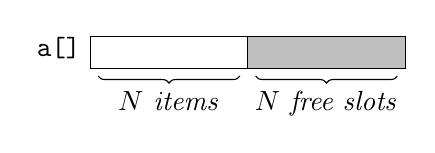
\begin{tikzpicture}
    \draw (0,0) 
          node[anchor=south east] {\texttt{a[]}}
          rectangle (2,.4);
    \draw [fill=gray!50] (2,0) rectangle (4,.4);
    \draw (1.9,-.1)[decorate, decoration=brace]
          -- node[below=2pt] {\textit{$N$ items}}
          (.1,-.1);
    \draw (3.9,-.1)[decorate, decoration=brace] 
          -- node[below=2pt] {\textit{$N$ free slots}} 
          (2.1,-.1);
  \end{tikzpicture}
  \caption{The data structure immediately after {\tt resize()}.}
\end{figure}



With this observation, we can proceed to show that at the start of
every subsequent call of {\tt resize()}, there are at least $4N$ coins
in the bank.
\begin{itemize}
\item If the call came from \texttt{push()}, i.e., to prevent
  overflow, then there must have been at least $N/2$ calls to
  \texttt{push()} since the last \texttt{resize()}. Each
  \texttt{push()} deposited 8 coins, so there are $4N$ coins, as
  needed.
\begin{figure}
  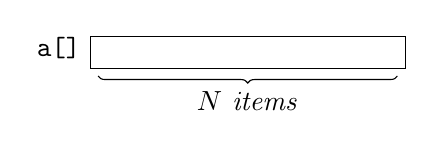
\begin{tikzpicture}
    \draw (0,0) 
          node[anchor=south east] {\texttt{a[]}}
          rectangle (4,.4);
    \draw (3.9,-.1)[decorate, decoration=brace]
          -- node[below=2pt] {\textit{$N$ items}}
          (.1,-.1);
  \end{tikzpicture}
  \caption{The data structure immediately before \texttt{push()} calls
    \texttt{resize()}.}
\end{figure}
\item If the call came from \texttt{pop()}, i.e., to prevent underflow,
  then there must have been at least $N$ calls to \texttt{pop()} since
  the last \texttt{resize()}. Each \texttt{pop()} deposited 4 coins,
  so there are $4N$ coins, as needed.
\begin{figure}
  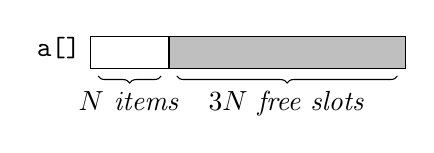
\begin{tikzpicture}
    \draw (0,0) 
          node[anchor=south east] {\texttt{a[]}}
          rectangle (1,.4);
    \draw [fill=gray!50] (1,0) rectangle (4,.4);
    \draw (0.9,-.1)[decorate, decoration=brace]
          -- node[below=2pt] {\textit{$N$ items}}
          (.1,-.1);
    \draw (3.9,-.1)[decorate, decoration=brace] 
          -- node[below=2pt] {\textit{$3N$ free slots}} 
          (1.1,-.1);
  \end{tikzpicture}
  \caption{The data structure immediately before \texttt{pop()} calls {\tt resize()}.}
\end{figure}
\end{itemize}
\end{proof}

\begin{ExerciseList}
  \Exercise \label{ex: only push}Can we charge all costs to
  \texttt{push()}? How much does it have to pay if \texttt{pop()} pays nothing?
  \Exercise Can we charge all costs to
  \texttt{pop()}? How much does it have to pay if \texttt{push()} pays nothing?
\end{ExerciseList}

\section{Localising the piggy bank argument}

Sometimes it is easier to localise the accounting argument by removing
the fictional piggy bank and depositing the coins in the data
structure instead.

For example, we can say that push operation puts 8 coins in the cell
it just filled, and every pop puts 4 coins in the cell that it just
freed. 

As before, when doubling the array from $N$ to $2N$, we argue that at
least $N$ {\tt push()} operations happened, so the entries in {\tt a}
from $N/2-1$ to $N$ contain at east 8 coins each, for a total of $4N$
coins. Similarly, for halving the array from $4N$ to $2N$, the calls
to {\tt pop()} put 4 coins on each of the free cells in $N+1,\ldots,
2N$, for a total of $4N$ coins. 

The local argument is sometimes attractive because there is a strong
inuition about what the coins will be doing, should they ever be
needed.  
For example, the 4 coins deposited by {\tt pop} in position {\tt
  a[N+1]} will be able to pay for the allocation of the new array
cells {\tt temp[1]} and {\tt temp[N+1]}, and the two accesses in {\tt
  temp[1] = a[1]}.

\begin{figure*}
  \tikzstyle{cell}=[draw,on chain,minimum width=6mm,
  font=\tiny\tt, text height=1.25ex, text depth=.25ex]
  \tikzstyle{coin}=[draw,circle, on chain,inner sep= 1pt, fill=white,font=\tiny\sf]
  \begin{tikzpicture}[node distance=0cm]
    \begin{scope}[start chain]
      \node[on chain] {\tt a};
      \foreach \word in {to, be, or, not} \node [cell] {\word};
      \foreach \i in {4,...,7} \node [cell] {\it null};
    \end{scope}
    \node at (6,-.5) [anchor=west]{\tt pop(); pop();} ;
    \begin{scope}[start chain]
      \node at (0,-1) [on chain] {\tt a};
      \foreach \word in {to, be} \node (a\word) [cell]{\word};
      \foreach \i in {2,...,7} \node [cell](C\i) {\it null};
    \end{scope}
    \begin{scope}[start chain= going {at=(\tikzchainprevious),shift=(-80:.3)}]
      \node (N21) [coin,below of=C2] {N};
      \node (N22) [coin] {N};
      \node (R2) [coin] {R};
      \node (W2) [coin] {W};
    \end{scope}
    \begin{scope}[start chain= going {at=(\tikzchainprevious),shift=(-80:.3)}]
      \node (N31) [coin, below of=C3] {N};
      \node (N32) [coin] {N};
      \node (R3) [coin] {R};
      \node (W3) [coin] {W};
    \end{scope}
      \node at (6,-2) (TEMP) [anchor=west]{\tt temp = };
    \begin{scope}[start chain]
      \chainin (TEMP);
      \node [draw, red, on chain] (NEW) {\tt new Object[4];};
    \end{scope}
    \begin{scope}[start chain]
      \node at (0,-3) [on chain] {\tt temp};
      \foreach \i in {0,...,3} \node (NN\i) [cell] {\it null};
    \end{scope}
    \node at (6,-3.5) (TEMP0) [anchor=west,draw]{\tt temp[0] };
    \begin{scope}[start chain]
      \chainin (TEMP0);
      \node [on chain] {\tt = };
      \node [on chain, draw, red] (A0) {\tt a[0];};
  \end{scope}
  \node at (6,-4.3) (TEMP1) [anchor=west,draw]{\tt temp[1] };
  \begin{scope}[start chain]
    \chainin (TEMP1);
    \node [on chain] {\tt = };
    \node [on chain, draw, red] (A1) {\tt a[1];};
  \end{scope}    
  \begin{scope}[start chain]
      \node at (0,-5) [on chain] {\tt temp};
      \node (to) [cell] {to};   \node (be) [cell] {be};
      \foreach \i in {2,...,3} \node [cell] {\it null};
    \end{scope}
    \draw [->,nearly transparent] (N21) to[out=0,in=135] (NEW);
    \draw [->,nearly transparent] (N22) to[out=0,in=135] (NEW);
    \draw [->,nearly transparent] (N31) to[out=0,in=135] (NEW);
    \draw [->,nearly transparent] (N32) to[out=0,in=135] (NEW);
    \draw [->,nearly transparent] (R2) to (TEMP0);
    \draw [->,nearly transparent] (R3) to (TEMP1);
    \draw [->,nearly transparent] (W2) to (A0);
    \draw [->,nearly transparent] (W3) to (A1);
  \end{tikzpicture}
  % 
  \caption{ Two {\tt pop()} operations each deposit 4 coins (marked N, N, R,
    W), in {\tt a[2]} and {\tt a[3]} respectively.  When {\tt
      resize()} is called, the coins marked N are spent allocated the
    new array {\tt temp}, the R coin is spent reading from {\tt a},
    and the W coin is spent writing to {\tt temp}. In the new {\tt a}
    (which is {\tt temp}), there is no money.  }
\end{figure*}

But it's a matter of taste. I like the local argument better for
exercise~\ref{ex: only push}.



\begin{ExerciseList}
\Exercise
Prove proposition~C using the piggy bank method instead.
If you use the local argument, where does the money go?
How little do you actually need?
\footnote{To make this entertaining, assume it takes one pound
  sterling to turn a wheel and give the answer in pence.
  Next, assume it takes 1 shilling.}
\Exercise
 Assume the counter is built out of increasingly heavy material. 
 Each wheel costs twice as much to turn as the previous.
 (So, turning wheel 0 costs 1, wheel 1 costs 2, wheel 2 costs 4, 
 $\ldots$,  wheel $k$ costs $2^k$.)
 Does the analysis still work?
 What if wheel $k$ costs $10^k$? $11^k$?
\end{ExerciseList}

\section{On the word `average' in [SW]}

We already discussed the use of the word `average' and its various meanings.
The concept described in these notes is a specific kind of average called `amortised,' and we have tried to be disciplined in our use of it.
This does not mean that the mental model of `amortisation is just some kind of average' is false.
In particular, the textbook [SW] itself uses the word in its own formulation of proposition A4.

However, as a possible source of confusion the word `average' is used in Proposition K in [SW, Sec. 2.3] with a different meaning:
\begin{quote}
  {\bf Proposition K}. Quicksort uses $\sim 2N\ln N$ compares (and one-sixth that many exchanges) on the average to sort an array of length $N$ with distinct keys.
\end{quote}
This statement describes the running time of a single run of an algorithm on a random input (namely, a sequence of uniformly and independently distributed integers).
This is precisely \emph{not} how `average' is used in proposition A4:
There, the sequence (which defines repeated operations on a data structure) is nonrandom (it is, in fact, a worst case sequence.)


\chapter{Union--Find Variants}

\begin{summary}
In this section we consider two variants of union--find, and present careful analyses of their amortised running times.

This makes sense after [SW] 1.5.
\end{summary}


The union--find analyses in this chapter serve primarily as examples of nontrivial applications of the aggregate method; the weighted quick-union structure is better than both of our variants in this section.
However, both data structures are examples of more general algorithmic design principles that are very useful in other contexts:
\begin{enumerate}
  \item if you have to update parts of a data structure, favour decision that update the \emph{smaller} part.
    This is the idea behind the \emph{weighted} version of quick-find.
  \item \emph{memoization}: if you've performed a computation, store its result, so as to avoid recomputing it later.
    This is the idea behind \emph{path compression}.
\end{enumerate}

Both of these ideas are intuitively clever, and worst-case analysis is unable to establish this intuition.
In contrast, the amortized analysis shows in both variants that they are worth doing.

\section{Weighted quick-find}

We return to the first, very simple union-find data structure of [SW],
called \emph{quick-find}. 

Let us try to salvage this idea, at least partially. We're not going
to be able to beat the quick-union implementations, but this section
is mainly about \emph{analysis}, not so much about presenting the best
union--find algorithm known to Man.

Our first improvement is to make a clever choice about whether
\texttt{union(p, q)} renames {\tt p}'s component to {\tt q}'s or vice
versa. 
Our choice is to always rename the smaller component.
For this, we introduce another array {\tt int[] sz} to store component sizes, initially all $1$, and with the same meaning as in algorithm~1.4.

The second improvement is to link all elements of a component, so that we can quickly iterate over them when we want to rename them, instead of iterating over all of {\tt id}.
For this, we implement yet another array {\tt int[] next} of indices,
so that {\tt next[i]} is the element following {\tt i} in some
circular list of the component ids.

For example, the data structure looks like this after the operations
described by {\tt tinyUF.txt}.:

\medskip
{\tt \small
  \begin{tabular}{rcccccccccc}
      & 0 & 1 & 2 & 3 & 4 & 5 & 6 & 7 & 8 & 9 \\\midrule
id[] & 6 &6 &6 &4 &4 &6 &6 &6 &4 &4 \\
next[] & 5 &2 &0 &4 &9 &6 &7 &1 &3 &8 \\
sz[] &1 &1 &3 &1 &4 &1 &6 &1 &1 &1 
  \end{tabular}}
\medskip

Figure \ref{fig: WUF} shows the this situation, and the situation
after another call to {\tt union()}. 
An implementation is given in figure~\ref{fig: WUF impl}.

\begin{figure}
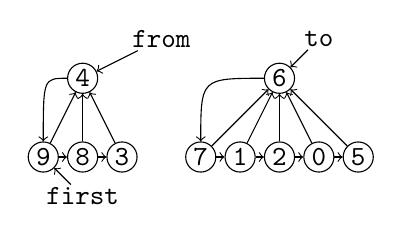
\begin{tikzpicture}[font=\tt,scale=.5,every node/.style={draw,circle,
    inner sep=1pt}]
  \node (9) at (0,0) {9};
  \node (8) at (1,0) {8};
  \node (3) at (2,0) {3};
  \node (4) at (1,2) {4};
  \foreach \x in {9,8,3} 
    \draw[->] (\x)--(4);

  \node (7) at (4,0) {7};
  \node (1) at (5,0) {1};
  \node (2) at (6,0) {2};
  \node (0) at (7,0) {0};
  \node (5) at (8,0) {5};
  \node (6) at (6,2) {6};
  \draw[->] (7)--(1);
  \draw[->] (1)--(2);
  \draw[->] (2)--(0);
  \draw[->] (0)--(5);
  \foreach \x in {7,1,2,0,5} 
    \draw[->] (\x)--(6);
  \draw[->] (6).. controls(4,2)..(7);
  \draw[->] (9)--(8);
  \draw[->] (8)--(3);
  \draw[->] (4)..controls(0,2)..(9);

  \node[draw=none,rectangle] at (1,-1) {first} edge [->] (9);
  \node[draw=none,rectangle] at (3,3) {from} edge [->] (4);
  \node[draw=none,rectangle] at (7,3) {to} edge [->] (6);
\end{tikzpicture}

\bigskip
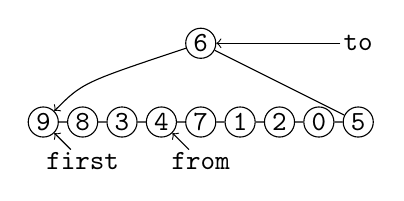
\begin{tikzpicture}[font=\tt,scale=.5,every node/.style={draw,circle,
    inner sep=1pt}]
  \node (9) at (0,0) {9};
  \node (8) at (1,0) {8};
  \node (3) at (2,0) {3};
  \node (4) at (3,0) {4};

  \node (7) at (4,0) {7};
  \node (1) at (5,0) {1};
  \node (2) at (6,0) {2};
  \node (0) at (7,0) {0};
  \node (5) at (8,0) {5};
  \node (6) at (4,2) {6};
  \draw[->]   (9)--(8)--(3)--(4)--(7)--(1)--(2)--(0)--(5)--(6)
  ..controls(1,1)..(9);

  \node[draw=none,rectangle] at (1,-1) {first} edge [->] (9);
  \node[draw=none,rectangle] at (4,-1) {from} edge [->] (4);
  \node[draw=none,rectangle] at (8,2) {to} edge [->] (6);
\end{tikzpicture}
\bigskip
\caption{\label{fig: WUF}{\tt union(1,8)}, where {\tt id[8] == 4} and {\tt id[1] ==
    6}.  The {\tt next} pointers are shown.}
\end{figure}


\begin{figure}
  \begin{tabbing}
   \quad\=\quad\=\quad\=\kill\\
    \textbf{public class} WeightedQuickFind \{\\
\>  private int[] id, sz, next;\\
\>  private int count;\\
\>\\
    \>  public WeightedQuickFind(int $N$)  \{\\
   \> \>    count = $N$;\\
    \>\>    id = new int[$N$];\\
    \>\>    next = new int[$N$];\\
    \>\>    sz = new int[$N$];\\
    \>\>    for (int $i$ = 0; $i$ < $N$; $i$++) \{ \\
\>\>\>      id[$i$] = $i$;\\
\>\>\>   next[$i$] = $i$;\\
    \>\>\>      sz[$i$] = 1;\\
\>\>    \}\\
\>  \}\\
\>\\
\>  private void rename(int from, int to) \{ \\
\>\>    int first = next[from];\\
    \>\>    for (int $i$ = first; $i$ != from; $i$ = next[$i$])\\
\>\>\>	id[$i$] = to;\\
\>\>    id[from] = to;\\
\> \>   next[from] = next[to];\\
\>  \>  next[to] = first;\\
\> \>   sz[to] += sz[from];\\
\>  \}\\
\>\\
\>  public void union(int $p$, int $q$) \{\\ 
    \>\>    int pID = find($p$); \\
\>\>    int qID = find($q$);\\
\>\>    if (pID == qID) return;\\
    \>\>    if (sz[pID] < sz[qID]) \= rename(pID,qID);\\
\>   \> else                  \> rename(qID,pID);\\
\>\>    count -= $1$;\\
\>  \}\\
\}
  \end{tabbing}
\caption{\label{fig: WUF impl}Weighted quick-find. 
  See [SW, sec. 1.5] for find.}
\end{figure}


Intuitively, we have made our data structure a lot faster.
For instance, consider the sequence of $N-2$ unions with arguments $(0,1)$, $(1,2)$, $(2,3)$, $\ldots$, $(N-2,N-1)$.
Each operations takes constant time, whereas the original {\tt QuickFind} data structure would have used linear time.
This is great progress.
Unfortunately, our usual way of analyses is unable to detect that improvement, because we usually are interested in \emph{worst-case} running times.
And the worst case running time of {\tt WeightedQuickFind} is quite bad:

\begin{ExerciseList}
  \Exercise{}\label{ex: quick-find worst case}
  Exhibit a call to {\tt union()} for which {\tt WeightedQuickFind} that takes linear time.

  \Answer{} Begin with $k-2$ calls to union with arguments $(0,2)$, $(1,3)$, $(2,4)$, $\ldots$, $(k-2, k)$.
  At this stage, all the odd elements are in their own component, and all the even elements are in their own component, each of size $\sim \frac12 k$.
  Now a single call to union$(0,1)$ will have to access $\sim12 k$ array elements of \texttt{id}.
\end{ExerciseList}

Again, the proper way to analyse the data structure is the amortized point of view.
\footnote{
  Before we continue, let's remind ourselves that there is a good reason for our usual focus on the worst case.
  We normally don't evaluate our data structure by its behaviour on particularly well-chosen inputs that make the data structure look good. 
  The \emph{best-case} time for {\tt QuickFind} was constant as well, after all: Just call {\tt union(0,1)} $N$ times in a row.

  Also note that `typical case' (however that should be defined) is a no-starter.
  Almost all calls to union in our two examples take constant time, so the `typical case behaviour is constant for {WeightedQuickFind}'---but that says more about our input sequences than the data structure.

  At this time one is tempted to define `average case,' or, to be quite precise `average input sequence.'
  This can indeed be done quite rigorously, by defining a random process.
  For instance, we could pick $p,q\in\{0,\ldots, N-1\}$ at random, independently and with the same probability, and then try to determine the expected value of the running time of {\tt union($p$,$q$)} after $N$ operations.
  There are two reasons for us to \emph{not} pursue this method of analysis.
  First, it is mathematically sophisticated and requires some exposure to discrete probability theory.
  Second, it tells us surprisingly \emph{little} about our data structure, because the result depends very heavily on the choice of distribution.
  (For instance, why should $p$ and $q$ be independent? 
  Why should they be uniformly distributed instead of normal, or Poisson, or a dozen other distributions that appear in real life?)
  To appreciate these questions, imagine the union--find data structure used in an algorithm for Kruskal's algorithm for minimum spanning tree.
  Then the $p$ and $q$ depend on the structure of the input graph and the weight of its edges---that is absolutely not a uniformly random process!
  It would be much more interesting to define, say `the input sequence arising from the union--find calls of an execution of Kruskal's algorithm on a random graph.'
  But this gets \emph{very} difficult to analyse (including specific details about the implementation of Kruskal!), and only shifts the question to `what kind or random process did the graph arise from'?
  No matter how we try to define `random inputs,' we find ourselves in the position of having to motivate the distribution.
  
  The discussion above largely served to motivate why we try to avoid the term `average.'
  It's not very well defined, and of very questionable value.
  (Moreover, we can't do the math.)
}


\begin{theorem}\label{thm: weighted quick-find amortized}
  In weighted quick-find for $n\geq 2$ elements, the {\tt union()} operation takes amortized time $O(\log n)$ in the worst case, beginning from an initialized data structure.
\end{theorem}

\begin{proof}
We can show this using the aggregate method, so we consider a sequence of $k$ calls to {\tt union()} and want to show that it takes $O(k\log n)$ time.

We will count the number of updates of {\tt id[]} in {\tt rename()}, from the perspective of a single site $i$. 
The crucial observation is that whenever the {\tt id} of $i$ is renamed, the size of its component at least doubles.
(This is because we always rename the smaller of two unioned components, and the size of the union is at least twice of the smaller one.)
On the other hand, no component can ever be larger than $n$. 
Thus, the component of $i$ has been doubled no more than $\log_2 n$ times.
In particular, {\tt id[i]} has been changed at most $\log_2 n$ times.

Next, we need to argue that at most $2k$ sites are ever renamed during the $k$ operations.
This is because a site that never appeared as one of the two arguments in some call to {\tt union} still remains in its original component.
Thus, at most $2k$ sites are ever renamed.
We argued above that each site gets renamed at most $\log n$ times in total.
Thus, the total number of updates to {\tt id} is at most $2k\log_2 n$. 
\end{proof}

Let us reiterate a few points about the formulation of Theorem~\ref{thm: weighted quick-find amortized}
\begin{enumerate}
  \item  Note the role that `worst case' plays:
    It says that in \emph{any}, even the most maliciously constructed input sequence, is is \emph{impossible} that the first $k$ operations take more than $O(k\log n)$ time in total.
    (Of course, the claim \emph{also} holds for `best case' or `average case' or `typical case', however you want to define them.
    But none of those statements are interesting, and all of them are weaker.)
\item Note the role that `amortized' plays:
  Without it, the theorem is plainly false; as shown by Exercise~\ref{ex: quick-find worst case}.
\item Note the role that `beginning from an initialized data structure' plays. 
  Without it, the claim is plainly false: if we begin later, Exercise~\ref{ex: quick-find worst case} shows that there are sequences of length $1$ (namely, \texttt{union(0,1)}) that take time linear in the size of the data structure.
    And if we begin earlier, then the initialisation itself takes time $O(n)$ already for $k=0$.
\end{enumerate}

\section{Unweighted Quick-Union with Path Compression}

Assume that we extend the (unweighted) quick-union algorithm (SW, pp. 224) to include \emph{path compression}, but not  union-by-rank.
To be precise, we rewrite the \texttt{find(int p)}-operation so that it links every site on the path from $p$ to the root directly to the root, like in Fig.~\ref{fig: path compression}

\begin{figure}[h]
  \[
  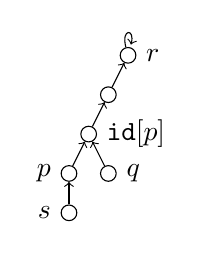
\begin{tikzpicture}[scale = .5]
  \node (p)    at (0,0) [circle, draw, inner sep = 2pt, label = left:$p$] {};
    \node (idp)  at (.5,1) [circle, draw, inner sep = 2pt, label = right:{$\mathtt{id}[p]$}] {};
  \node (dots) at (1,2) [circle, draw, inner sep = 2pt] {};
  \node (r)    at (1.5,3) [circle, draw, inner sep = 2pt, label = right:$r$] {};
    \node (q) at (1,0) [circle, draw, inner sep = 2pt, label = right:$q$] {};
    \node (s) at (0, -1) [circle, draw, inner sep = 2pt, label = left:$s$] {};
  \draw [->] (p) -- (idp);
  \draw [->] (q) -- (idp);
  \draw [->] (idp) -- (dots);
  \draw [->] (dots) -- (r);
    \draw[->] (s) -- (p);
  \path [->] (r) edge [loop above] (r);
\end{tikzpicture}
\quad
\text{is `shortcut' into}
\quad
  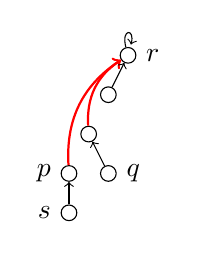
\begin{tikzpicture}[scale = .5]
  \node (p)    at (0,0) [circle, draw, inner sep = 2pt, label = left:$p$] {};
  \node (idp)  at (0.5,1) [circle, draw, inner sep = 2pt] {};
    \node (dots) at (1,2) [circle, draw, inner sep = 2pt] {};
  \node (r)    at (1.5,3) [circle, draw, inner sep = 2pt, label = right:$r$] {};
    \node (q) at (1,0) [circle, draw, inner sep = 2pt, label = right:$q$] {};
    \node (s) at (0, -1) [circle, draw, inner sep = 2pt, label = left:$s$] {};
    \path [->,thick, red] (p) edge[bend left] (r);
    \path [->,thick, red] (idp) edge[bend left] (r);
  \draw [->] (dots) -- (r);
  \path [->] (r) edge [loop above] (r);
  \draw [->] (q) -- (idp);
    \draw[->] (s) -- (p);
\end{tikzpicture}
\]
  \caption{\label{fig: path compression}
  Path compression resulting from the call \texttt{find($p$)}.
  The edges on the path from $p$ to the root $r$, except for the last edge, are removed and replaced by new edges (shown red.)
  The resulting distance to the root for every node on the path is now $1$.
  }
\end{figure}
The idea is that since the algorithm is `touching' each of these nodes anyway, it might as well spend slightly more time shortcutting them to link directly to the root, so that \emph{next} time they'll be close to it.

One elegant way of implementing that is recursively, as follows:
\begin{quote}
\begin{tabbing}
  $\quad$\=\kill
  \textbf{public int} find(\textbf{int} $p$) \{\\
  \>  \textbf{if} (id[$p$] == $p$) \textbf{return} $p$;\\
  \>  \textbf{int} $r$ = find(id[$p$]);\\
\>  id[$p$] = $r$;\\
  \>  \textbf{return} $r$;\\
  \}
\end{tabbing}
\end{quote}

\begin{ExerciseList}
  \Exercise{} 
  Give a nonrecursive implementation of the same idea. 
\end{ExerciseList}

We will show that this data structure is as good as \emph{weighted} quick-union, at least in the amortised sense:

\begin{theorem}[Exercise 1.5.12 in SW]\label{prop: path compression}
  (Unweighted) quick-union on a universe of $n\geq 2$ elements with path compression takes $O(\log n)$ amortised time per update in the worst case.
\end{theorem}

Before proving this, convince yourself that amortisation is crucial for this claim.
For unlike for weighted quick-union, we cannot establish a logarithmic time bound \emph{in the worst case}:

\begin{ExerciseList}
  \Exercise{} Exhibit a sequence of operations (unweighted) quick-union with path compression where a single operation requires linear time, $\Theta(n)$.
  \Answer{}  Begin with $n$ unions
  \texttt{union($0$,$1$)}, 
  \texttt{union($1$,$2$)}, 
  $\ldots$, 
  \texttt{union($n-2$,$n-1$)}.
  (Each took constant time, the data structure is now a directed path of length $n$.)
  Now call \texttt{find($0$)}.
  This single operation requires linear time, so the worst case time for an operation is (at least) linear.
\end{ExerciseList}

\begin{proof}[Proof of Prop.~\ref{prop: path compression}]
  We need to consider an arbitrary sequence of $k$ operations (unions or finds) and show that the total time for these operations is $O(k\log n)$.

  Our cost model will be the total number of edges, not including self-loops, that are destroyed by find operations at any time during the evolution of the data structure.
  This choice requires some attention.
  Each \emph{union} operation performs a nontrivial but constant amount of work, in total $O(k)$, which we can neglect compared to $O(k \log n)$.
  (This includes destroying self-loops.)
  Each \emph{find} operation performs a constant amount of work (mainly traversing edges), again at most $O(k)$ in total.
  Whenever a \emph{find} operation traverses \emph{more} than a single edge, it immediately performs a path compression that \emph{destroys} those edges (except the last one.)
  Thus, we can restrict our attention to counting destroyed edges---they exactly correspond to the nonconstant work performed by \emph{find}, everything else costs $O(k)$ in total.

  \medskip

  We let $T_u$ denote the subtree rooted at node $u$, including $u$ itself.
  An edge $e$ from $u$ to $v$ (with $u\neq v$) is called \emph{heavy} if, at the time of its destruction, it accounted for at least half of its parent's weight in the sense that $|T_u| \geq \frac12|T_v|$.
  Otherwise it is \emph{light}.
  We will show that both the number of light edges and the number of heavy edges are at most $O(k\log n)$.

  \medskip
  \emph{Light:}
  Consider a particular \emph{find} operation and let $v_1$, $\ldots$, $v_r$ be the path of vertices traversed by the operation, numbered from bottom to top.
  Let $e$ from $u$ to $v$ be a light edge on this path.
  Because $e$ is light, the corresponding subtrees double in size: $|T_v| > 2|T_u|$.
  Thus, if the path contains $l$ light edges, we have \[|T_{v_r}| > 2^l |T_{v_1}|\,.\]
  Since $|T_{v_r}|\leq n$ and $|T_{v_1}| \geq 1$, we have $l\leq\log_2 n$.
  Thus, the path contains at most $\log_2 n$ light edges, and therefore the \emph{find} operation cannot destroy more than that many.
  Since there are at most $3k$ \emph{find} operations, we conclude that the total number of light edges destroyed is $O(k\log n)$.
 
  \medskip
  \emph{Heavy:}
  We count the heavy edges by associating each heavy edge $e$ from $u$ to $v$ with its target endpoint $v$.
  Let $e_1,\ldots, e_r$ be the heavy edges pointing to $v$ at any time during the evolution of the data structure.
  Let $w_1,\ldots, w_r$ denote the \emph{weight} of $v$, i.e., the size $|T_v|$ of the subtree rooted at $v$, at the time when $e_1,\ldots, e_r$ were destroyed.

  A crucial observation is that at the time $t$ when $e_1$ was destroyed, vertex $v$ was no longer a root.
  (Path compression never manipulates the last edge on a path, so only non-roots can get  incoming edges removed.)
  Thus, $v$ never \emph{gains} weight after time $t$.
  Moreover, because each $e_i$ is heavy, we know that the removals of $e_1$, $\ldots$, $e_r$ each reduced the weight of $v$ by at least half.
  Thus, 
  \[ w_1\geq 2 w_2 \geq 2^2w_3\cdots\geq 2^{r-1} w_r\,.\]
  Since each $w_i$ is an integer between $1$ and $n$, we have $r - 1\leq \log_2 n$.
  There are at most $2k$ different target vertices (vertices that were never an argument to \emph{union} have no incoming edges except their own self-loop), so the total number of heavy edges is $O(k\log n)$.
\end{proof}

\begin{ExerciseList}
  \Exercise{}
  The idea of \emph{path halving} is a simpler version of path compression. 
  The find operation merely connects every vertex to its granparent on the path, instead of to the root.
  Does the above proof still apply?
  \Answer{}
  Almost.
  The cost model is still valid, since number of edges still accounts for the number of operations, up to linear terms.
  But it is less clear that a vertex only ever loses weight after it ceases to be a root.
  (After all, path halving may connect a vertex to a fresh parent that is not a root.)
  However, it is true that no vertex ever receices a new \emph{descendant} after it loses its self-loop, so the main argument remains true and the proof can be fixed.
\end{ExerciseList}


\section{Weighted Quick--Union with Path Compression}

As before, consider a sequence of $k$ many interleaved union- and find-operations on a data structure for universe size $n$.
As before, note that the number of nodes ever accessed by the $k$ operations is $O(\min\{2k, n\})$.
As before, let $T_u$ denote the subtree rooted at $u$.


\subsection{Rank}

Let $R_u$ be the largest subtree of $u$ at any time during the evolution of the data structure.

(To gain some inuition, it can be seen that while $u$ is a root its subree only ever grows, namely when other trees are linked below $u$ after a \emph{union}, and after $u$ ceases to be a root its subtree only ever shrinks, namely when its descendants are moved to new parents by a path compression.
Thus, $R_u$ is the subtree $T_u$ immediately before the union-operation that makes $u$ a non-root.)

Define the \emph{rank} of $u$ to be \[ r_u= \left\lfloor \log_2 |R_u|\right\rfloor\,\]
and note 
\[ r_u\in\{0,\ldots, \lfloor\log_2 n\rfloor \}\,.\]

\begin{lemma}[Invariant: ranks strictly increase along edges]%
  \label{lem:ranksincrease}
  Assume $uv$ for $u\neq v$ is an edge at any time during the data structure.
  Then $r_u<r_v$.
\end{lemma}

\begin{proof}
  Consider the edges $uv$ in the order they are created during the $k$ operations.

  The first edge $uv$ is the result of the first union operation \emph{union}$(u,v)$.
  Node $u$ ceases to be a root, so $r_u = \lceil \log_2 1\rceil =0$, and $|R_v|\geq |T_v| =2$, so $r_v\geq 1$.
  More generally, let $uv$ be a new edge.
  If $uv$ is the result of a union then $u$ and $v$ are both roots.
  Let $T_u$ and $T_v$ be the trees rooted at $u$ immediately before the operation,
  note that they are disjoint because $u$ and $v$ are both roots.
  By the weighting strategy, $|T_u|\leq |T_v|$.
  Node $u$ just ceased to be a root, so $R_u= T_u$ and its rank is $r_u =\lfloor \log_2 |T_u| \rfloor$.
  After the operation, $v$ is still a root and is now the ancestor of all the elements in $T_u$ and $T_v$.
  It may gain even more descendants later, but certainly $|R_v|\geq |T_u| + |T_v| \geq 2|T_u|$.
  In particular
  \[ 
    r _v = 
    \lfloor\log R_v\rfloor  =
    \lfloor\log_2 2|T_u|\rfloor =
    \lfloor 1 + \log_2 |T_u|\rfloor = 
    1 + \lfloor\log_2 |T_u|\rfloor =
    1 + \lfloor\log_2|R_u|\rfloor = 1 + r_u\,,
    \]
  so $u$ has strictly higher rank than $v$.

  If $uv$ is the result of a path compression then there is a path from $u$ along already existing edges to a root $v'$.
  The root $v'$ has higher rank than $u$ by induction, and we can replace $v$ by $v'$ in the above argument.
\end{proof}

\begin{lemma}[parent rank strictly increases over time]%
  \label{lem:parentrank}
  Assume the edge $uv$ with $u\neq v$ is replaced by the edge $uw$. 
  Then $r_u<r_w$.
\end{lemma}
\begin{proof}
  When $u$ is not a root then it gains a new parent $w$ only by path compression.
  The compressed path necessarily includes the edge $uv$ and ends at $w$.
  In particular, $w$ is an ancestor of $v$, so $r_w>r_v$ by the previous lemma.
\end{proof}

\begin{lemma}
  If $u$ and $v$ with $u\neq u$ have the same rank then $R_u$ and $R_v$ are disjoint.
\end{lemma}
\begin{proof}
  Consider $w$ belonging to both $R_u$ and $R_v$.
  One of $u$ and $v$, say $u$, becomes a non-root first.
  (If both $u$ and $v$ are roots at the end, then $R_u$ and $R_v$ are obviously disjoint no matter their ranks.)
  When $v$ becomes an ancestor of $w$, it is also an ancestor of $u$.
  Thus $r_v>r_u$ by Lemma~\ref{lem:ranksincrease}, so that $u$ and $v$ do not have the same rank.
\end{proof}

Let $n_r$ be the number of nodes of rank $r$ ever accessed by the operations.

\begin{lemma}\label{lem:n_r}
  \[ n_r \leq \frac{k}{2^r}\,.\]
\end{lemma}
\begin{proof}
  For every node $u$ of rank $r$, the tree $R_u$ has size  \[|R_u|= 2^{\log_2|R_u|} \geq 2^{\lfloor \log_2|R_u|\rfloor} = 2^r\,,\] and they are all disjoint according to the above lemma.
\end{proof}

\subsection{Tower function}

\begin{definition}[Tower function]
  Define the tower function $t$ for each nonnegative integer by 
  \[t(i) = \begin{cases}
    1\,,& i =0\,;\\
    2^{t(i-1)}\,,& i >0\,.\\
  \end{cases}
  \]
\end{definition}

Here are the first few values of $t(0), t(1),\ldots$:

\begin{tabular}{ccccccccc}
  $i$ & 0 & 1 & 2 & 3 & 4 & 5& 6 & $\cdots$ \\
  $t(i)$ & 1 & 2 & 4 & 16 & 65536 & $2^{65536}$ & $2^{2^{65536}}$ & $\cdots$
\end{tabular}

The tower sequence grows quickly---the decimal representation of $t_5$ has $19,729$ digits yet can still be written down on half a page of paper; whereas $t_6$ has more digits than there are protons in the known universe.

The inverse of the tower sequence is the iterated logarithm.
\begin{definition}[Iterated logarithm]
  For $n\geq 0$ define
  $\log^* n =  \min\{\, i \colon t(i) \geq n\}$.
\end{definition}

For instance, $\log^* 3= 2$, $\log^* 4 = 3$, and $\log^* 100,000 = 4$.
In particular, if $n<10^{100}$ is the number of atoms in the universe (a reasonable upper bound on a realistic input size) then $\log^* n =5$.
However, formally $\log^* n$ is \emph{not} bounded by a constant, and we have $\log^* n \notin O(1)$.

\subsection{Rank group}

The nodes in the data structures are partitioned into groups according to their rank:
\begin{definition}[Rank group]
  For $i\in \{0,\ldots, \log^*n\}$, the node $u$ belongs to rank group $G_i$ if $t(i-1) < r_u \leq t(i)$.
\end{definition}

The core structural insight is that the rank groups decrease in size dramatically.

\begin{lemma}
  \[|G_i| \leq \frac{k}{2^{t(i)}}\,.\]
\end{lemma}
\begin{proof}
  For $a<b$ the number of nodes of rank $r$ with $a< r\leq b$ is, by Lemma~\ref{lem:n_r},
  \[ n_{a+1} +\cdots + n_b \leq \frac{k}{2^{a+1}} + \cdots + \frac{k}{2^b} =
  k\left(\frac{1}{2^{a+1}} + \cdots + \frac{1}{2^b}\right) \leq
  k\cdot \frac{1}{2^a}\,.
  \]
  In particular, the number of nodes in rank group $i$ is at most $2^{t(i-1)} = t(i)$.
\end{proof}

\subsection{Analysis}

It suffices to count the edges along paths traversed by \emph{find} operations.
Consider an edge $uv$ along such a path.
By Lemma~\ref{lem:ranksincrease}, the ranks along the path strictly increase.
At most $\log^* n$ edges can cross a rank group (there are at most that many rank groups.)
Summing over all $k$ many \emph{find} operations, there are at most $k\log^* n$ such edges in total.

It remains to count, for vertex $u$, the number of edges $uv$ ever traversed by a find operation such that $v$ belongs to the same rank group as $u$.
Except for the last edge along a compressed path, each of these edges gets destroyed by this traversal.

\begin{lemma}
  Let $u$ be a node in rank group $G_i$.
  The number of destroyed edges $uv$ with $v\neq u$ and $v\in G_i$ is at most $t(i)$.
\end{lemma}
\begin{proof}
  Let $v_1,\ldots, v_s$ be the nodes such that $uv_j$ is ever an edge, and let $r_1, \ldots, r_s$ be their ranks.
  Whenever $u$s parent changes from root $v_j$ to new root $v_{j+1}$, their rank increases by Lemma~\ref{lem:parentrank}.
  Thus, the ranks are all different yet belong to $G_i$, so there can be at most $t(i)-t(i-1)\leq t(i)$ many.
\end{proof}

Summing over all $u\in G_i$ we get that the number of destroyed edges $uv$ with $u,v\in G_i$ is
\[ \frac{k}{t(i)}t(i) =k\,. \]
There are at most $\log^*n$ rank groups, so the total contribution is $k\log^*n$.

In total, the number of edges ever traversed is $O(k + k\log^* n)$.

\appendix
\chapter{Answers}

\shipoutAnswer

\end{document}
